\section{Material and methods}
\subsection{Software development}
A simulation of the combined model can take several minutes. The thereafter calculation and handling of these results are not granted to work in the process of a program development. We designed a simple workflow that prevents to repeat a simulation with already simulated settings:
\begin{enumerate}
	\item simulation $\Rightarrow$ save data
	\item fetch data $\Rightarrow$ analysis
\end{enumerate}
For the construction of this workflow a PostgreSQL database was implemented and connected with the python script. Pure python3 code was the choice for this thesis.  \\
A concept from CDISC for clinical trials was used for the data storing architecture. This allows to construct useful column names, data types and table in the database.\\ 
Because a simulation of ODEs and algebraic equations can have pending sets of initial values, parameter values or equations terms, the concept of CDISC was expanded to the area of system biology by designing new data storage procedures. This helps to keep track for all model settings and changes and use any of them for a new simulation. The intention for the  implementation of CDISC to system biology was the fact, that the FDA is moving towards CDISC standards for regulatory submissions \cite{SDTMStandard}. \\
In figure \ref{proposedWorkflow} we can see  the proposed workflow.
\begin{figure}[h!]
	\begin{center}
		\begin{minipage}{0,8\textwidth}
			
			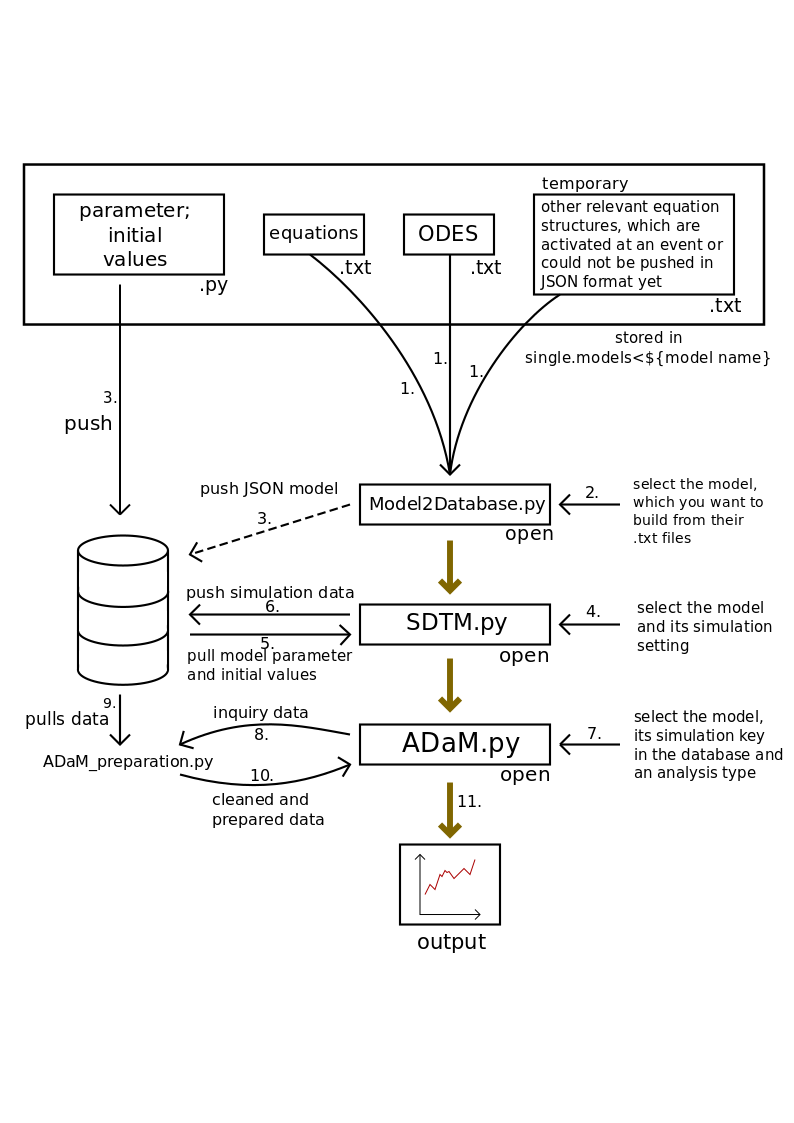
\includegraphics[width=\textwidth]{picture/proposedWorkflow.png}
			\caption{workflow for the analysis of a model in the designed software} 
			\label{proposedWorkflow} 
		\end{minipage}
	\end{center}
\end{figure}\\\\
With this approach, we can analysis and try new codes snippets with the results of a long simulation in few seconds. \\
Furthermore, the storage of the model in a JSON file was designed in a way, that a natively typed equation in a .txt file format like 
\begin{equation*}
	\frac{d}{dt} Na_{in} = \frac{J_{Na} \cdot G}{V_{os}} \cdot 10^6 - Na_{in} \cdot V_{ratio} 
\end{equation*}
gets automatically separated in the terms $\frac{J_{Na} \cdot G}{V_{os}} \cdot 10^6$ and $- Na_{in} \cdot V_{ratio}$. This allows us to simulate each term component and analyze its contribution to the result of the equation in relation to the time.\\
\newpage